% Options for packages loaded elsewhere
\PassOptionsToPackage{unicode}{hyperref}
\PassOptionsToPackage{hyphens}{url}
%
\documentclass[
]{book}
\usepackage{lmodern}
\usepackage{amssymb,amsmath}
\usepackage{ifxetex,ifluatex}
\ifnum 0\ifxetex 1\fi\ifluatex 1\fi=0 % if pdftex
  \usepackage[T1]{fontenc}
  \usepackage[utf8]{inputenc}
  \usepackage{textcomp} % provide euro and other symbols
\else % if luatex or xetex
  \usepackage{unicode-math}
  \defaultfontfeatures{Scale=MatchLowercase}
  \defaultfontfeatures[\rmfamily]{Ligatures=TeX,Scale=1}
\fi
% Use upquote if available, for straight quotes in verbatim environments
\IfFileExists{upquote.sty}{\usepackage{upquote}}{}
\IfFileExists{microtype.sty}{% use microtype if available
  \usepackage[]{microtype}
  \UseMicrotypeSet[protrusion]{basicmath} % disable protrusion for tt fonts
}{}
\makeatletter
\@ifundefined{KOMAClassName}{% if non-KOMA class
  \IfFileExists{parskip.sty}{%
    \usepackage{parskip}
  }{% else
    \setlength{\parindent}{0pt}
    \setlength{\parskip}{6pt plus 2pt minus 1pt}}
}{% if KOMA class
  \KOMAoptions{parskip=half}}
\makeatother
\usepackage{xcolor}
\IfFileExists{xurl.sty}{\usepackage{xurl}}{} % add URL line breaks if available
\IfFileExists{bookmark.sty}{\usepackage{bookmark}}{\usepackage{hyperref}}
\hypersetup{
  pdftitle={DMAC Training Modules},
  pdfauthor={Kyle Roell, Lauren Koval, Julia Rager},
  hidelinks,
  pdfcreator={LaTeX via pandoc}}
\urlstyle{same} % disable monospaced font for URLs
\usepackage{longtable,booktabs}
% Correct order of tables after \paragraph or \subparagraph
\usepackage{etoolbox}
\makeatletter
\patchcmd\longtable{\par}{\if@noskipsec\mbox{}\fi\par}{}{}
\makeatother
% Allow footnotes in longtable head/foot
\IfFileExists{footnotehyper.sty}{\usepackage{footnotehyper}}{\usepackage{footnote}}
\makesavenoteenv{longtable}
\usepackage{graphicx,grffile}
\makeatletter
\def\maxwidth{\ifdim\Gin@nat@width>\linewidth\linewidth\else\Gin@nat@width\fi}
\def\maxheight{\ifdim\Gin@nat@height>\textheight\textheight\else\Gin@nat@height\fi}
\makeatother
% Scale images if necessary, so that they will not overflow the page
% margins by default, and it is still possible to overwrite the defaults
% using explicit options in \includegraphics[width, height, ...]{}
\setkeys{Gin}{width=\maxwidth,height=\maxheight,keepaspectratio}
% Set default figure placement to htbp
\makeatletter
\def\fps@figure{htbp}
\makeatother
\setlength{\emergencystretch}{3em} % prevent overfull lines
\providecommand{\tightlist}{%
  \setlength{\itemsep}{0pt}\setlength{\parskip}{0pt}}
\setcounter{secnumdepth}{5}
\usepackage{booktabs}
\usepackage[]{natbib}
\bibliographystyle{plainnat}

\title{DMAC Training Modules}
\author{Kyle Roell, Lauren Koval, Julia Rager}
\date{2021-06-03}

\begin{document}
\maketitle

{
\setcounter{tocdepth}{1}
\tableofcontents
}
\hypertarget{introduction}{%
\chapter{Introduction}\label{introduction}}

The UNC-Superfund Research Program (SRP) seeks to develop new solutions for reducing exposure to inorganic arsenic and prevent arsenic-induced diabetes through mechanistic and translational research.

The Data Analysis and Management Core (DMAC) provide the UNC-Superfund Research Program with critical expertise in bioinformatics, statistics, data management and data integration. Our goal is to support the data management, integration, and analysis needs of the researchers to reveal multi-factorial determinants of inorganic arsenic-induced metabolic dysfunction/diabetes.

\hypertarget{intro}{%
\chapter{Setting Up Your R Environment}\label{intro}}

R is a free, open source programming language

\begin{itemize}
\tightlist
\item
  Anyone can download and use

  \begin{itemize}
  \tightlist
  \item
    Doesn't require a license
  \item
    Good for reproducible analyses
  \end{itemize}
\item
  Large, diverse collection of packages
\item
  Comprehensive documentation
\end{itemize}

\hypertarget{r-and-rstudio}{%
\section{R and RStudio}\label{r-and-rstudio}}

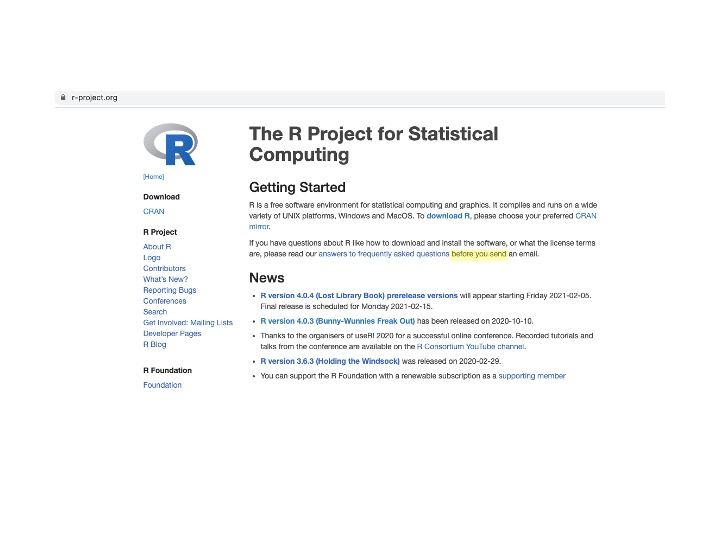
\includegraphics{test1_files/figure-html/Rager_RIntro_Resources.jpg}

\hypertarget{downloading-r-and-rstudio}{%
\subsection{Downloading R and RStudio}\label{downloading-r-and-rstudio}}

\hypertarget{installing-r-and-rstudio}{%
\subsection{Installing R and RStudio}\label{installing-r-and-rstudio}}

\hypertarget{installing-and-loading-packages}{%
\subsection{Installing and Loading Packages}\label{installing-and-loading-packages}}

\hypertarget{scripting-basics}{%
\section{Scripting Basics}\label{scripting-basics}}

\hypertarget{setting-working-directory}{%
\subsection{Setting Working Directory}\label{setting-working-directory}}

\hypertarget{importing-and-exporting-files}{%
\subsection{Importing and Exporting Files}\label{importing-and-exporting-files}}

\hypertarget{viewing-data}{%
\subsection{Viewing Data}\label{viewing-data}}

\hypertarget{dataorg}{%
\chapter{The Basics for Data Organization}\label{dataorg}}

\hypertarget{basic-data-manipulation}{%
\section{Basic Data Manipulation}\label{basic-data-manipulation}}

\hypertarget{merging}{%
\subsection{Merging}\label{merging}}

\hypertarget{merging-processed-data-with-metadata-file}{%
\subsection{Merging processed data with metadata file?}\label{merging-processed-data-with-metadata-file}}

\hypertarget{cast}{%
\subsection{Cast}\label{cast}}

\hypertarget{melt}{%
\subsection{Melt}\label{melt}}

\hypertarget{filtering-subsetting}{%
\subsection{Filtering \& subsetting}\label{filtering-subsetting}}

\hypertarget{tidyverse-stuff-pivots}{%
\subsection{Tidyverse stuff (pivots)}\label{tidyverse-stuff-pivots}}

\hypertarget{finding-and-visualizing-data-trends}{%
\chapter{Finding and Visualizing Data Trends}\label{finding-and-visualizing-data-trends}}

\hypertarget{heat-maps}{%
\section{Heat maps}\label{heat-maps}}

\hypertarget{pheatmap}{%
\subsection{pheatmap}\label{pheatmap}}

\hypertarget{heatmap2}{%
\subsection{heatmap2}\label{heatmap2}}

\hypertarget{superheat}{%
\subsection{superheat}\label{superheat}}

\hypertarget{clustering}{%
\section{Clustering}\label{clustering}}

Examples with genomics: Rager et al.~2014

\hypertarget{hierarchical}{%
\subsection{Hierarchical}\label{hierarchical}}

\hypertarget{k-means}{%
\subsection{K-means}\label{k-means}}

\hypertarget{data-reduction-pca}{%
\section{Data reduction (PCA)}\label{data-reduction-pca}}

\hypertarget{visualize-pca-plot}{%
\subsection{Visualize PCA Plot}\label{visualize-pca-plot}}

\hypertarget{identify-of-variance-captured}{%
\subsection{Identify \% of variance captured}\label{identify-of-variance-captured}}

\hypertarget{basic-statistical-tests-and-visualizations-of-data}{%
\section{Basic Statistical Tests and Visualizations of Data}\label{basic-statistical-tests-and-visualizations-of-data}}

Need an example dataset -- maybe ELGAN shuffled/deidentified, with made-up environmental exposure column?

\hypertarget{normality}{%
\subsection{Normality}\label{normality}}

Kruskal wallis? The other one that I always forget? Shapiro wilks? - histogram

\hypertarget{t-tests-column-charts}{%
\subsection{T-tests -- column charts}\label{t-tests-column-charts}}

\hypertarget{regression-linear-regression-and-logistic-regression}{%
\subsection{Regression: linear regression and logistic regression}\label{regression-linear-regression-and-logistic-regression}}

\hypertarget{anova-delicate-commentary}{%
\subsection{ANOVA + delicate commentary}\label{anova-delicate-commentary}}

\hypertarget{chi-squared-test-box-plots}{%
\subsection{Chi-squared test -- box plots}\label{chi-squared-test-box-plots}}

\hypertarget{fishers-exact-test}{%
\subsection{Fisher's exact test}\label{fishers-exact-test}}

\hypertarget{multi-omics-analyses-for-environmental-health}{%
\chapter{Multi-Omics Analyses for Environmental Health}\label{multi-omics-analyses-for-environmental-health}}

\hypertarget{exposomics}{%
\section{Exposomics}\label{exposomics}}

\hypertarget{placenta-exposome}{%
\subsection{Placenta Exposome}\label{placenta-exposome}}

about to be submitted to EI
Dust NTA data

\hypertarget{transcriptomics}{%
\section{Transcriptomics}\label{transcriptomics}}

\hypertarget{deseq2-rnaseq}{%
\subsection{DESeq2 / RNAseq}\label{deseq2-rnaseq}}

Wildfire dataset, available through GEO

\hypertarget{genome-wide-microrna}{%
\section{Genome-wide MicroRNA}\label{genome-wide-microrna}}

Rager et al.~2014 miRNAs

\hypertarget{genome-wide-dna-methylation}{%
\section{Genome-wide DNA Methylation}\label{genome-wide-dna-methylation}}

\hypertarget{illumina-array-data}{%
\subsection{Illumina array data}\label{illumina-array-data}}

\begin{verbatim}
https://www.ncbi.nlm.nih.gov/geo/query/acc.cgi?acc=GSE58499
https://www.ncbi.nlm.nih.gov/geo/query/acc.cgi?acc=GSE28368
\end{verbatim}

\hypertarget{proteomics}{%
\section{Proteomics}\label{proteomics}}

\begin{verbatim}
Bailey et al arsenic dataset maybe?
\end{verbatim}

\hypertarget{mixtures-analyses-for-environmental-health}{%
\chapter{Mixtures Analyses for Environmental Health}\label{mixtures-analyses-for-environmental-health}}

\hypertarget{sufficient-similarity}{%
\section{Sufficient Similarity}\label{sufficient-similarity}}

Botanicals example with chemistry and tox profiling -- Julia has dataset

\hypertarget{mixtures-modeling-through-qgcomp}{%
\section{Mixtures Modeling through qgcomp}\label{mixtures-modeling-through-qgcomp}}

Could use published wildfire analysis here (Rager et al.~2021, STOTEN), or online example provide through Alex Keil's studies

\hypertarget{environmental-health-databases}{%
\chapter{Environmental Health Databases}\label{environmental-health-databases}}

\hypertarget{comparative-toxicogenomics-database-ctd}{%
\section{Comparative Toxicogenomics Database (CTD)}\label{comparative-toxicogenomics-database-ctd}}

\hypertarget{gene-expression-omnibus-geo}{%
\section{Gene Expression Omnibus (GEO)}\label{gene-expression-omnibus-geo}}

\hypertarget{nhanes}{%
\section{NHANES}\label{nhanes}}

\end{document}
